\documentclass[a4paper,12pt]{article}
\usepackage[T1]{fontenc}
\usepackage[utf8]{inputenc}
\usepackage{mathtools}
\usepackage[italian]{babel}
%\usepackage{graphicx}
\usepackage{float}
\usepackage{textcomp}
\usepackage{amsmath}

\title{Esercitazione 4}
\author{Olivieri Daniele}
\date{}

\begin{document}
\maketitle
In un serbatoio è contenuta dell'aria ad una pressione $p_a$ di 2.58 bar ed una temperatura $T_a$ di 378 K. La pressione ambiente $p_2$ è di 1 bar.
\begin{enumerate}
    \item Valutare le trasformazioni che avvengono in uno stadio di turbina assiale nel quale espande il suddetto fluido, nell'ipotesi
    di trasformazioni adiabatiche isoentropiche e flusso monodimensionale.
    In particolare si valuti lo stato termodinaico statico e totale monte/valle statore e monte/valle rotore. Si consideri sia uno stadio ad azione
    ed uno a reazione (triangoli delle velocità "simmetrici")    
    \item Calcolare il salto entalpico disponibile, $\Delta h^*$   
    \item Calcolare il lavoro ricavato dalla turbina
    \item Calcolare il rendimento di palettatura
    \item Valutare e disegnare i triangoli delle velocità
    \item Rappresentare sul piano T-s ed h-s le trasformazioni
    \item Disegnare le palettature statoriche e rotoriche
\end{enumerate}
Si assuma un angolo tra la velocità assoluta all'uscita dello statore e la direzione tangenziale $\alpha_1$ di 15°
\section{Analisi condizioni termodinamiche}
\label{sec:analisi_termodinamiche}
Il gas si trova inizialmente alle condizioni di ristagno (A), supposta nulla la velocità all'interno del serbatoio, espande isoentropicamente fino alla pressione di 1 bar
attraverso uno stadio di turbina che ne ricaverà dunque del lavoro da tale espansione. Non conoscendo le dimensioni del serbatoio o la massa di gas possiamo fare
solo ragionamenti per unità di massa.
Considerando la trasformazione isoentropica possiamo facilmente calcolare lo stato termodinamico 2 in uscita dalla turbina.
\begin{equation}
    \label{eq:isoentropica}
    T_2 = T_a\cdot\beta^{\frac{1-k}{k}}
\end{equation}
con $\beta$ pari a 2.58 e $k$ pari a 1.4, la temperatura in uscita dalla turbina varrà 288.3 K, con l'ausilio dell'equazione di stato dei gas
\begin{equation}
    \label{eq:stato_gas}
    pv = RT
\end{equation}
possiamo quindi completare la tabella con gli stati termodiamici a monte e a valle della turbina.

\begin{center}
    \begin{tabular}{c|c|c|c}
        Stato   &p (bar)    &T (°C) &v ($m^3/kg$) \\ \hline
        A       &2.58       &104,8  &0.420  \\
        2       &1          &15.2   &0.827  
    \end{tabular}
\end{center}
Il salto entalpico specifico disponibile $\Delta h^*$ è quindi pari a $C_p \cdot (T_1-T_2)$ ossia 90.12 kJ/kg

\section{Stadio ad azione}
\label{sec:stadio_ad_azione}
Consideriamo in prima analisi uno stadio ad azione, l'espansione del gas avviene nelle palette statoriche che trasformano tutta l'energia di pressione in velocità,
essendo ferme non producono ovviamente lavoro, si individua quindi una condizione termodinamica intermedia tra statore e rotore nella quale la pressione è identica
alla pressione in uscita ma l'energia cinetica ha eguagliato l'energia potenziale (ossia l'entalpia totale $\Delta h^*$) posseduta in precedenza dal gas.
\begin{equation}
    \label{eq:entalpia_stadio_azione}
    \Delta h^* = \frac{c_1^2}{2}
\end{equation}
quindi
\begin{equation}
    \label{eq:vel_stadio_azione}
    c_1 = \sqrt{2\Delta h^*}    
\end{equation}
$c_1$ = 424.5 m/s

Il gas deve essere quindi rallentato fino alla velocità $c_2$ dalle palette rotoriche per poter ottenere un lavoro utile, per massimizzare tale lavoro la velocità
in uscita dalla turbina deve essere la minima possibile ma al limite diversa da zero per conservare la condizione di flusso stazionario (non può esserci accumulo).
Il lavoro ottenuto dall'espansione sarà quindi
\begin{equation}
    \label{eq:lavoro_ad_azione}
    l = \Delta h^* - \frac{c_2^2}{2}
\end{equation}

Sia $\vec u$ la velocità tangenziale del rotore, $\vec c$ la velocità assoluta del fluido rispetto ad un sistema inerziale esterno alla turbina,
risulterà $\vec w$ la velocità relativa del fluido rispetto alla palettatura e pari quindi a  $\vec c - \vec u$.
Questi tre vettori formano un \textbf{triangolo delle velocità} e permettono un'analisi rapida del moto del fluido attraverso le palettature,
supponiamo quindi di costruire la turbina in maniera ottimale, limitando il più possibile il modulo delle velocità per ridurre al minimo le perdite.
% dovute alla viscosità del fluido.
Per ricavare la velocità tangenziale $\vec u_1$ della turbina ad azione possiamo utilizzare la seguente relazione
\begin{equation}
    \left.\frac{u_1}{c_1}\right|_{opt} = \frac{\cos \alpha_1}{2}
\end{equation}
L'angolo $\alpha_1$ varia generalmente tra i 10 e i 20 gradi al fine di ottenere rendimenti elevati, un angolo troppo elevato delle palette sstatoriche rallenta poco 
il fluido, un angolo troppo piccolo richiederebbe dimensioni maggiori della palettatura per consentire una pari portata.
Nel testo dell'esercizio quest'angolo viene richiesto uguale a 15° quindi $|\vec u_1|$ sarà pari a 205 m/s e uguale anche a $|\vec u_2|$ per la rigidità
del rotore.

Supponiamo ora che la velocità in uscita dal rotore sia parallela all'asse della turbina, sarà quindi pari a
\begin{equation}
    c_2 = c_1 \cdot \sin \alpha
\end{equation}
ossia 109.9 m/s.

Utilizzando la \eqref{eq:vel_stadio_azione} possiamo infine calcolare il lavoro ricavato dall'espansione: 84.08 kJ/kg con un rendimento del 93.3 \%.
Con l'ausilio di \textit{GeoGebra} possiamo facilmente disegnare i due triangoli impostando i parametri $\alpha_1$ e $\Delta h^*$
\begin{figure}[H]
    \label{fig:triangoli_azione}
    \centering
    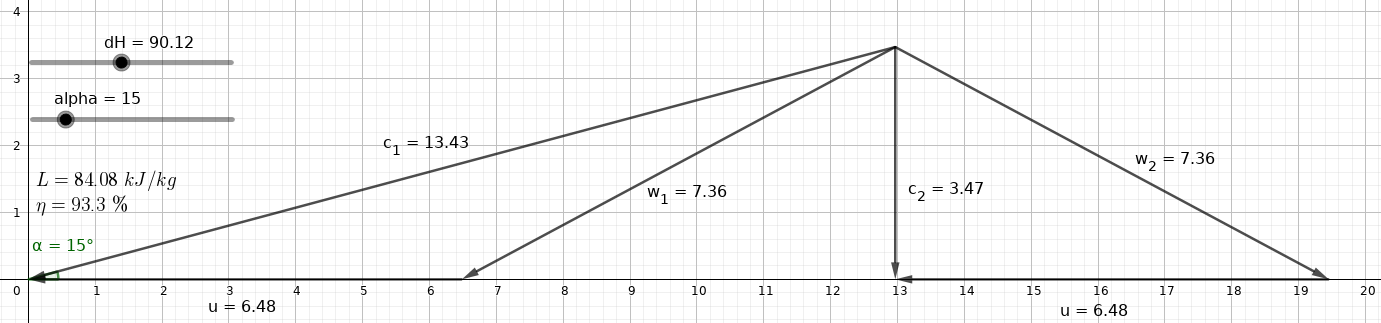
\includegraphics[width=\linewidth]{media/triangoli_azione.png}
\end{figure}
e misurare le lunghezze dei vettori.

\section{Stadio a reazione}
\label{sec:stadio_a_reazione}
Non siamo costretti a far espandere il fluido interamente nello statore, è possibile costruire uno stadio detto a \textbf{reazione} compiendo una espansione parziale
nello statore e la rimanente differenza di pressione verrà trasformata in lavoro nella successiva palettatura rotorica.
Si definisce \textbf{grado di reazione} il rapporto:
\begin{equation}
    \label{eq:grado_di_reazione}
    R \stackrel{def}{=} \frac{\Delta h_{\text{rot}}}{l} = \frac{\frac{w_2^2-w_1^2}{2} + \frac{u_1^2 - u_2^2}{2} }  %numeratore
                                                                {\frac{c_1^2-c_2^2}{2} + \frac{w_2^2-w_1^2}{2} + \frac{u_1^2 - u_2^2}{2}}  %denominatore
\end{equation}
Volendo suddividere equamente i contributi di energia meccanica ricavati nel rotore tra la variazione di velocità assoluta e quella relativa al rotore stesso
posso costruire uno stadio con grado di reazione pari a 0.5.
La \eqref{eq:entalpia_stadio_azione} diventa
\begin{equation}
    \frac{c_1^2}{2} = \Delta h^* (1-R)
\end{equation}
diventa immediato il calcolo di $c_1$ pari a 300 m/s.
I triangoli di velocità sono ottimizzati se $c_2$ è parallelo all'asse del rotore ed uguale a $w_1$, la velocità del rotore $u$ sarà dunque
\begin{equation}
    u = c_1 \cdot \cos \alpha
\end{equation}
e pari a 290 m/s.
Seguendo i passaggi precedenti è possibile rappresentare quindi i triangoli di velocità
\begin{figure}[H]
    \label{fig:triangoli_reazione}
    \centering
    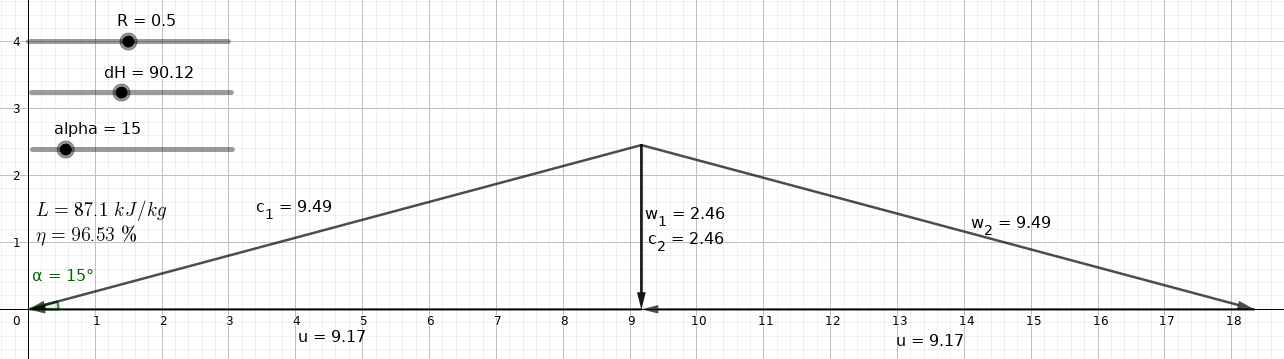
\includegraphics[width=\linewidth]{media/triangoli_reazione.png}
\end{figure}
Il lavoro ricavato dallo stadio a reazione si calcola allo stesso modo del caso precedente e risulta pari a 87.1 kJ/kg, il rendimento è quindi maggiore dello stadio
ad azione (96.5\%). Di contro la velocità tangenziale della turbina è aumentata notevolmente, ciò può causare uno stress eccessivo alle palette soggette ad un'elevata
forza centrifuga.

Conoscendo la velocità $c_1$ è possibile valutare lo stato termodinamico intermedio tra la palettatura statorica e quella rotorica con la \eqref{eq:entalpia_stadio_azione}
dato che ancora il lavoro ricavato nello statore è nullo.
Conoscendo la variazione di entalpia si ricava la variazione di temperatura dividendo per il $C_p$, si ricava $\beta$ dalla \eqref{eq:isoentropica}
ed applicando la \eqref{eq:stato_gas} determiniamo lo stato intermedio 1.

\begin{center}
    \begin{tabular}{c|c|c|c}
        Stato   &p (bar)    &T (°C) &v ($m^3/kg$) \\ \hline
        A       &2.58       &104,8  &0.420  \\
        1       &1.66       &60     &0.576  \\
        2       &1          &15.2   &0.827  
    \end{tabular}
\end{center}

Considerato un valore di riferimento per l'entropia, è possibile rappresentare le trasformazioni isoentropiche sul piano T-S, dove sono segnati i 3 stati termodinamici
appena ricavati, nel caso della turbina ad azione il punto 1 coincide con il punto 2 come già anticipato.
%Si può vedere come le aree delle due espansioni parziali siano praticamente uguali
\begin{figure}[H]
    \label{fig:trasformazioni_TS}
    \centering
    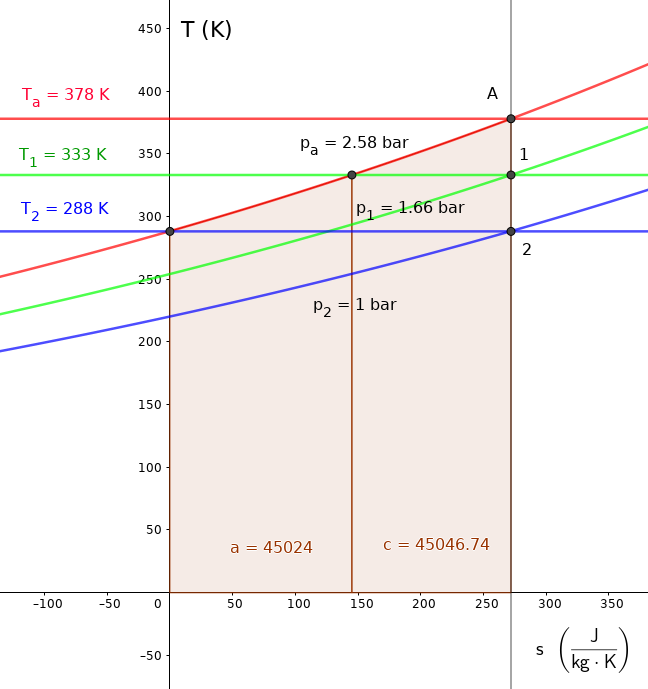
\includegraphics[width=.55\linewidth]{media/trasformazioni_TS.png}
\end{figure}

\end{document}
